\chapter{Methods\label{methods}}
This chapter aims to establish a precisely defined and rigorous research approach to enhance transparency and repeatability. We will take the steps required to ensure that every phase and decision is thoroughly documented, enabling the reader to retrace the research process. In a thesis made by a single researcher the lack of cross-examination of results with multiple researchers and the validation of evaluation criteria for opinion bias pose threats to validity, as will be clarified further in \hyperref[discussion]{Chapter 4}. Therefore, special attention will be paid to address these concerns. By following this approach, this research endeavors to contribute to the existing body of knowledge in the field of computer science in a robust and reliable manner.

The systematic literature review method (SLR) is a well-established approach for conducting a comprehensive and rigorous analysis of the existing research on specific research question or subject \citep{kitchenham2007}. This paper presents a multivocal literature review (MLR). MLR is a SLR that includes both academic (AL) and grey literature (GL). This method was selected for this study to facilitate a thorough and scientifically interdisciplinary examination of PCLs in software engineering. The existing literature consists of PCLs and as such are considered gray literature, making the thesis a multivocal literature review.

This study follows the guidelines outlined by \cite{kitchenham2007}, to ensure its quality. The multivocal review method consists of three distinct phases: planning, conducting and reporting the review. This study stricly adhered to this structure. The phases can be further broken down into a research protocol, as illustrated in \hyperref[fig:slrphases]{Figure 2.1}. Adhering to the protocol is the first step in ensuring a well-documented and rigorous process, which increases the validity and auditability of the study.

\begin{figure}
	\centering
	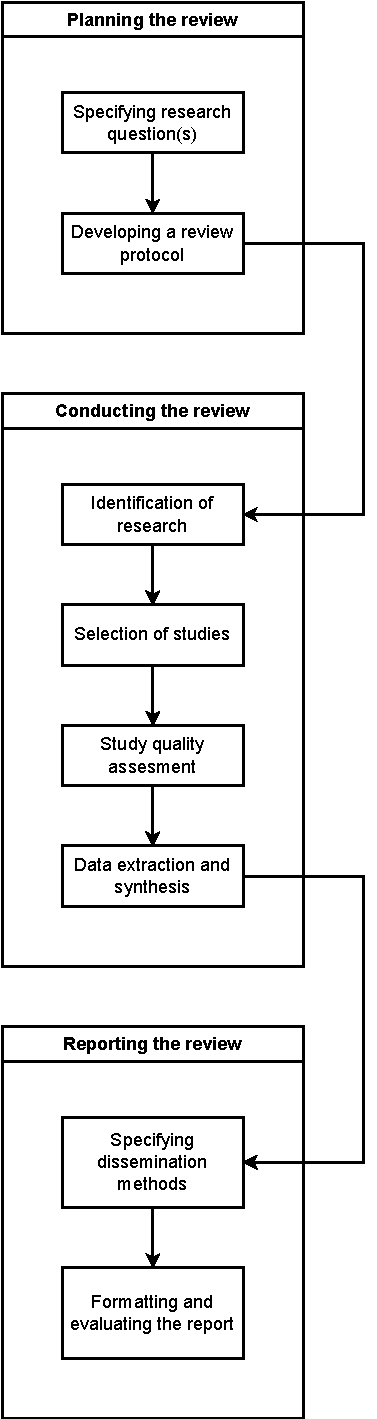
\includegraphics[scale=0.9]{figures/slr-phases.pdf}
	\caption{Three phases of a systematic literature review}
	\label{fig:slrphases}
\end{figure}

The multivocal literature review process began with the formulation of research questions and the establishment of a comprehensive search strategy and scope. The search process was conducted by employing a quasi-gold standard (QGS) approach based on the implementation by \cite{qgs}. After the completion of the search process, the inclusion and exclusion criteria were defined. To ensure a structured evaluation of the literature, a data extraction form was created. Finally, a strategy for analyzing the extracted data from the literature was designed.

 To ensure the reliability and validity of the research protocol, it was validated against similar systematic literature reviews in computer science, the aforementioned guidelines by \cite{kitchenham2007}, and was further refined through an iterative process. Specifically, a subset of the data was tested on (The QGS) and any identified issues or problems were recorded and addressed. The details of this process are explained and thoroughly documented in the following sections. Similarly, the same approach was followed for the data extraction process, whereby a subset of literature was tested to refine the data extraction form. The revision of the form was undertaken as necessary to guarantee the completeness and accuracy of the extracted data.

\section{Research questions}
The research questions in this study served two primary purposes. Firstly, they aimed to provide an anaylsis of the existing multivocal literature on PCLs in software engineering for the researchers interested about the field. Secondly, the questions were designed to cater a secondary audience of professional software engineering practicioners. As discussed in the \hyperref[intro]{Chapter 1}, the following research questions were addressed in this thesis:

\begin{itemize}
	\item RQ1: How many PCLs in software engineering does there exist?
	\item RQ3: What is the average length of a PCL in software engineering?
	\item RQ3: What are the most common components seen in PCLs in software engineering?
	\item RQ4: What are the most common changes made to PCLS in software engineering?
\end{itemize}

The multivocal literature review in this thesis begins with addressing RQ1, which aims to provide the amount of PCLs that exist in software engineering. The review takes into account attributes like versions, supersedences to a different license family, formal or otherwise and recognizability. These attributes give us different amounts to existing PCLs in software engineering. This information could be most valuable for the practicioners out of all the research questions in the thesis since it could give some sense of the scale when picking a PCL that would serve the practicioners' needs the best.

Next RQ2 seeks to find the average length of the text of a PCL in software engineering. This research question has attributes like the number of characters, sentences, distinct sections and the size of the license on a computer screen. This information could be valuable for the practicioners mentioned in the previous parapgrah for the same reasons of getting a better overview of the PCLs in software engineering. The research questions could also be beneficial for the practicioners working directly within the meta plane of PCLs in software engineering. Let us refer to the latter as researchers.

Finally RQ3 and RQ4 attempt to distinguish the top level paragraphs and other components of the PCLS in software engineering and what are the common reasons for the changes made to them throughout the years. The research questions go over the content of the changes and the implied and expressed reasons for making the changes. The answers to these last two research questions could again be useful for the researchers. The results can be used to introduce some notable background of the current PCLs in software engineering and enabling focus to more specific areas inside this PCLs in software engineering.

\section{Search stragey}
The search process was conducted on various PCL listing websites. The selection criteria for the literature were defined after the search process and the selection process was based on inclusion and exclusion criteria. The inclusion and exclusion criteria and each step of exclusion on the literature found was documented and is available as \hyperref[appendix:a]{Appendix A}. The used criteria are presented later in this chapter.

The data extraction process was performed in a standardized and systematic manner, with the aim of obtaining all relevant information from the selected literature. The data extraction form used included information such as license name, release year, text length and inferred purpose and is available  \hyperref[table:extraction]{Table 2.2}. The extracted data was then used to answer the research questions and perform the data analysis. The results of the data analysis were then reported in a rigorous manner.
\subsection{Search method}
The search was conducted on various PCL listing websites, as mentioned earlier, to obtain a broad set of multivocal literature. This approach yielded a large number of literature that were processed to a subset of high-relevance literature using exclusion and quality criteria presented later in this chapter. Manual searching of databases with thousands of PCLs is not feasible, and it is prone to researcher bias and may overlook relevant venues from other scientific disciplines. However, a preliminary manual search was performed to reduce the number of iterations required and establish the quasi-gold standard (QGS) mentioned earlier.
\subsection{Search scope and terms}
Originally the search terms would have been present just like in a normal MLR or SLR. Keywords however produced highly varying and non-reproducabe results in Google Scholar and Google Search. Some PCL listing websites such as FSF's list of pages categorized as licenses could not be found from Google Search even with the \texttt{site} operator: \texttt{site:https://directory.fsf.org/wiki/Category:License}. Although the page has been up since 2013 for some reason Google has not crawled the page in 10 years \citep{fsf:licenselist}. Hence why this thesis does not include search terms per se.

Instead, for establishing a QGS we started defining our search scope from the Wikipedia page of one of the most used open source license according to \cite{github:licenseusage}, the MIT license \citep{wikipedia:mit}. The infobox contained fields in the order shown in \hyperref[table:infobox]{Table 2.1}.

\begin{table}[t]
	\begin{center}
		\begin{tabular}{||c c||}
			\hline
			Field & Value \\
			\hline
			Publisher & Massachusetts Insitute of Technology \\
			SPDX identifier & MIT \\
			Debian FSG compatible & Yes \\
			FSF approved & Yes \\
			OSI approved & 	Yes \\
			GPL compatible & Yes \\
			Copyleft & No \\
			Linking from code with a different license & Yes \\
			\hline
		\end{tabular}
		\caption{MIT License Wikipedia page infobox}
		\label{table:infobox}
	\end{center}
\end{table}

As we defined PCLs in software engineering as copyright licenses where the licensees are not limited and the copyright license in question is meant be used in licensing software source code in \hyperref[methods]{Chapter 2} and our research questions focus on finding measurements and reasonings to the PCLs' various attributes, we decided to gather PCLs from the related web pages of the aforementioned categorizers: SPDX, FSF, OSI and GNU. The publisher, GPL compatibility, copyleft and the linking exception did not result in any meaningful PCL listing websites. This leaves us with the SPDX, Debian FSG compatibility, FSF and OSI from which all resulted in some sort of PCL listing websites.

With the search for the initial PCL listing websites completed we moved onto the search process itself.

\section{Search process}
The literature selection process was divided into multiple stages, as outlined in \hyperref[fig:search-process]{Figure 2.2}. The initial step involved the formation of the first PCL listing websites through which the first literature would be acquired from.

\begin{figure}
	\centering
	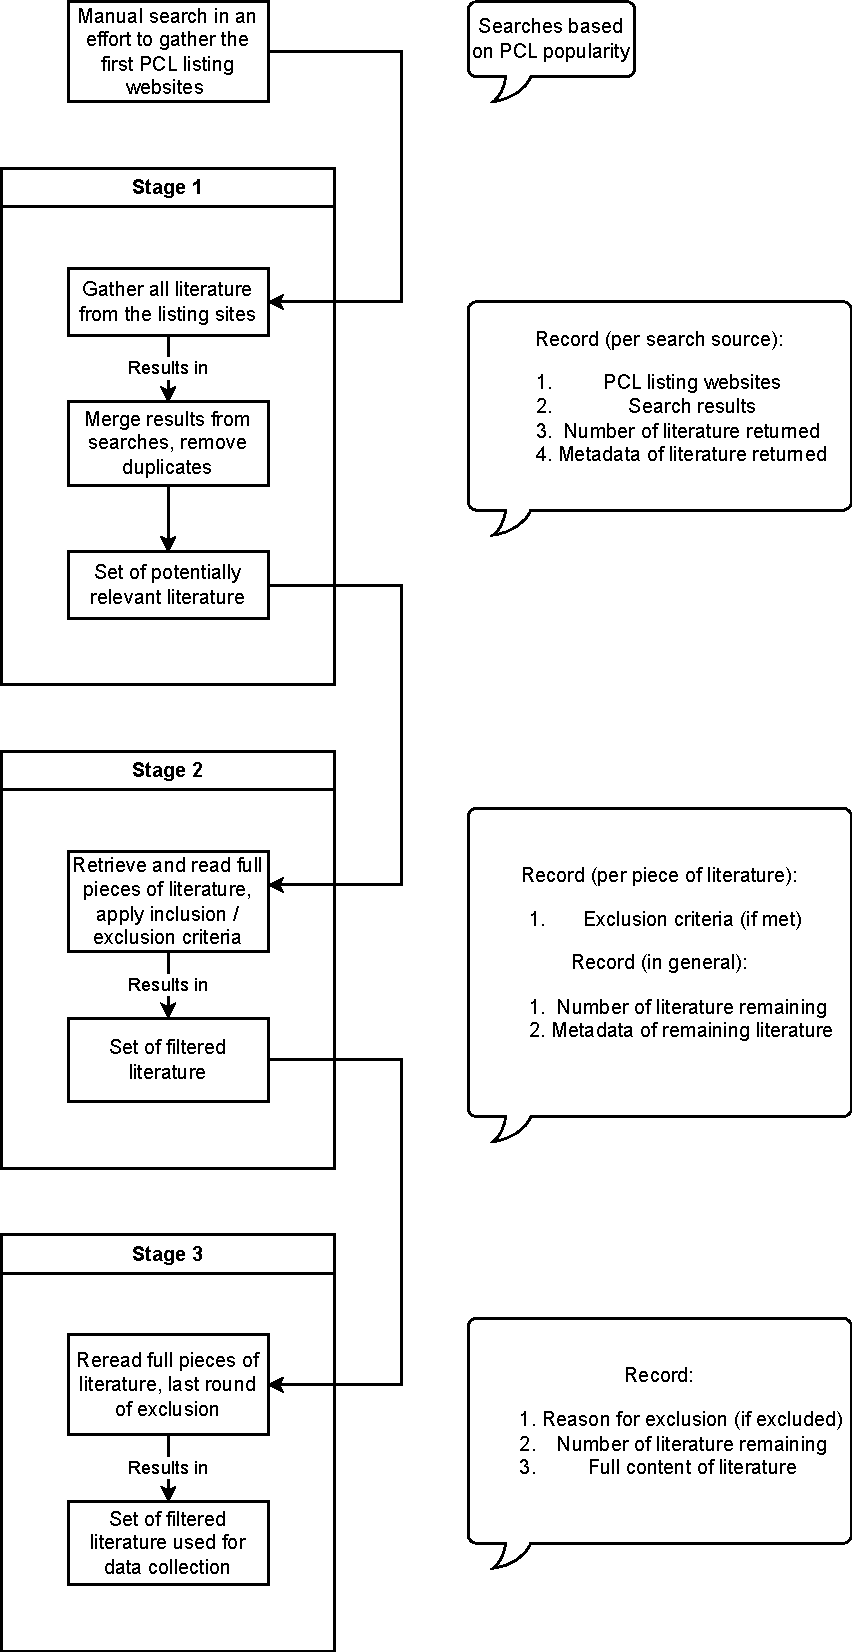
\includegraphics[scale=0.67]{figures/search-process.pdf}
	\caption{Search process divided into stages}
	\label{fig:search-process}
\end{figure}


In the first stage, the search was conducted using the ''SPDX License List'' \citep{spdx:licenses}, ''The DFSG and Software Licenses'' \citep{debian:dfsg}, FSF's ''Category:License'' Wiki page \citep{fsf:licenselist}, GNU's ''Various Licenses and Comments about Them'' \citep{gnu:licenselist} and "OSI Approved licenses" \citep{osi:licenselist}.

In the second stage, the inclusion and exclusion criteria were applied to further filter the literature and reduce the number of licenses to be reviewed. The exclusion reason as a shortcode (e.g. I1 = failed to meet inclusion criteria 1 or E2 = met exclusion criteria 2) is provided in \hyperref[appendix:a]{Appendix A}

The third stage was the most time-consuming and involved a manual review of the full licenses. After reading and evaluating each license, a final round of exclusions was completed and documented. The remaining licenses were used for data collection and analysis in the final part of the study. The final list of licenses is available in \hyperref[appendix:b]{Appendix B}.

\section{Inclusion and exclusion criteria}
To be eligible for the data collection and analysis, a license had to meet all of the following inclusion criteria:

\begin{itemize}
	\item I1: The license focuses mostly on the copyright of software source code
	\item I2: \textcolor{red}{inclusion criteria 2}
\end{itemize}

Additionally, licenses were excluded if they met any of the following criteria:

\begin{itemize}
	\item E1: The piece of literature is a license exception
	\item E2: \textcolor{red}{exclusion criteria here}
	\item E3: \textcolor{red}{exclusion criteria here}
	\item E4: \textcolor{red}{exclusion criteria here}
\end{itemize}

The relevance of each piece of literature was evaluated based on inclusion and exclusion criteria stated above. In cases where there was doubt about the suitability of a license, a more in-depth manual examination of its content was performed. The reason for exclusion was documented for each license that failed to meet the criteria, and when it was unclear, the license was included by default.

Another relevant criteria related to the ones of inclusion and exclusion are the quality and evidence criteria. These criteria used by \cite{dyba2007} were not put into practice in this thesis since individual PCLs per se might not be meaningful in a results, evidence nor quality perspective. This puts more emphasis on the inclusion and exclusion criteria so that is something we must be mindful about.

\section{Data collection and data analysis}
To answer the research questions of this thesis, a thorough examination of the selected primary literature was conducted and the necessary data was collected using data extraction form presented in \hyperref[table:extraction]{Table 2.2}. A record of extracted data was kept for anaysis and is available as \hyperref[appendix:b]{Appendix B}.

\begin{table}[t]
	\begin{center}
		\begin{tabular}{||c c c||} 
			\hline
			\# & Field & Concern/Research question \\
			\hline
			F1 & Name & Documentation \\
			F2 & Length & RQ3 \\
			F3 & FSF approval &  Documentation\\
			F4 & OSI approval & Documentation \\
			F5 & Inferred purpose & RQ1, RQ2, RQ4 \\
			\hline
		\end{tabular}
		\caption{Data extraction form}
		\label{table:extraction}
	\end{center}
\end{table}

The subsequent chapter presents the outcomes of the steps taken in the study, as discussed above.